\clearpage
\CourseSection{Readability Pilot}\label{app:readability-pilot}

We ran the readability method on the official 13,000-skill GitSkills sample to check that it is feasible and to choose the preprocessing.
Of the 13,000 distinct skills, 237 were not named exactly \texttt{SKILL.md}, 1,566 had invalid front matter, 555 were too short (a body under 300 characters or fewer than 30 words of prose), and 2,328 were not in English.
This left 8,314 skills from 5,567 repositories.
Figure~\ref{fig:readability-pilot}a shows why the Markdown must be converted into sentences before scoring: on raw text, each bullet list counts as one long sentence, and the median grade rises from 8.6 to 12.2.
Figure~\ref{fig:readability-pilot}b shows that skill sentences are short (a median of 9 words), but formulas that weight word length, such as Coleman--Liau, place the same text near grade 13, which reflects technical vocabulary.
Descriptions are usually a single long sentence, and they read about four grades harder than the bodies.
The pilot code uses textstat~\cite{textstat}; whole-sample scoring took about 6\,ms per skill on one laptop core, or roughly 3\,h for the full 1.88 million distinct skills.

\begin{figure}[htbp]
\centering
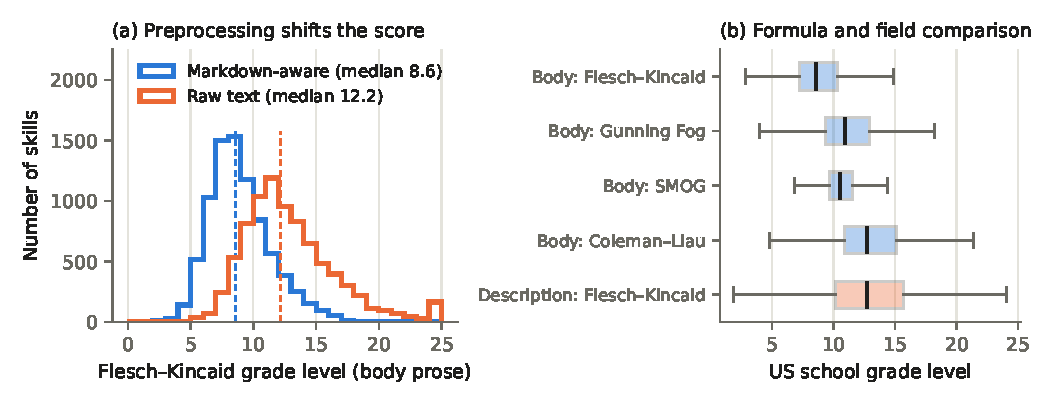
\includegraphics[width=\linewidth,keepaspectratio]{figures/readability-pilot.pdf}
\caption{Readability pilot on 8,314 English skills from the 13,000-skill GitSkills sample. (a)~Flesch--Kincaid grade of the body prose, with the Markdown converted to sentences and as raw text. (b)~Body grade under four formulas, and Flesch--Kincaid grade of the front-matter description. Boxes show the interquartile range, and whiskers extend to 1.5 times the IQR.}
\label{fig:readability-pilot}
\end{figure}
